
% Default to the notebook output style

    


% Inherit from the specified cell style.




    
\documentclass[11pt]{article}

    
    
    \usepackage[T1]{fontenc}
    % Nicer default font (+ math font) than Computer Modern for most use cases
    \usepackage{mathpazo}

    % Basic figure setup, for now with no caption control since it's done
    % automatically by Pandoc (which extracts ![](path) syntax from Markdown).
    \usepackage{graphicx}
    % We will generate all images so they have a width \maxwidth. This means
    % that they will get their normal width if they fit onto the page, but
    % are scaled down if they would overflow the margins.
    \makeatletter
    \def\maxwidth{\ifdim\Gin@nat@width>\linewidth\linewidth
    \else\Gin@nat@width\fi}
    \makeatother
    \let\Oldincludegraphics\includegraphics
    % Set max figure width to be 80% of text width, for now hardcoded.
    \renewcommand{\includegraphics}[1]{\Oldincludegraphics[width=.8\maxwidth]{#1}}
    % Ensure that by default, figures have no caption (until we provide a
    % proper Figure object with a Caption API and a way to capture that
    % in the conversion process - todo).
    \usepackage{caption}
    \DeclareCaptionLabelFormat{nolabel}{}
    \captionsetup{labelformat=nolabel}

    \usepackage{adjustbox} % Used to constrain images to a maximum size 
    \usepackage{xcolor} % Allow colors to be defined
    \usepackage{enumerate} % Needed for markdown enumerations to work
    \usepackage{geometry} % Used to adjust the document margins
    \usepackage{amsmath} % Equations
    \usepackage{amssymb} % Equations
    \usepackage{textcomp} % defines textquotesingle
    % Hack from http://tex.stackexchange.com/a/47451/13684:
    \AtBeginDocument{%
        \def\PYZsq{\textquotesingle}% Upright quotes in Pygmentized code
    }
    \usepackage{upquote} % Upright quotes for verbatim code
    \usepackage{eurosym} % defines \euro
    \usepackage[mathletters]{ucs} % Extended unicode (utf-8) support
    \usepackage[utf8x]{inputenc} % Allow utf-8 characters in the tex document
    \usepackage{fancyvrb} % verbatim replacement that allows latex
    \usepackage{grffile} % extends the file name processing of package graphics 
                         % to support a larger range 
    % The hyperref package gives us a pdf with properly built
    % internal navigation ('pdf bookmarks' for the table of contents,
    % internal cross-reference links, web links for URLs, etc.)
    \usepackage{hyperref}
    \usepackage{longtable} % longtable support required by pandoc >1.10
    \usepackage{booktabs}  % table support for pandoc > 1.12.2
    \usepackage[inline]{enumitem} % IRkernel/repr support (it uses the enumerate* environment)
    \usepackage[normalem]{ulem} % ulem is needed to support strikethroughs (\sout)
                                % normalem makes italics be italics, not underlines
    \usepackage{mathrsfs}
    

    
    
    % Colors for the hyperref package
    \definecolor{urlcolor}{rgb}{0,.145,.698}
    \definecolor{linkcolor}{rgb}{.71,0.21,0.01}
    \definecolor{citecolor}{rgb}{.12,.54,.11}

    % ANSI colors
    \definecolor{ansi-black}{HTML}{3E424D}
    \definecolor{ansi-black-intense}{HTML}{282C36}
    \definecolor{ansi-red}{HTML}{E75C58}
    \definecolor{ansi-red-intense}{HTML}{B22B31}
    \definecolor{ansi-green}{HTML}{00A250}
    \definecolor{ansi-green-intense}{HTML}{007427}
    \definecolor{ansi-yellow}{HTML}{DDB62B}
    \definecolor{ansi-yellow-intense}{HTML}{B27D12}
    \definecolor{ansi-blue}{HTML}{208FFB}
    \definecolor{ansi-blue-intense}{HTML}{0065CA}
    \definecolor{ansi-magenta}{HTML}{D160C4}
    \definecolor{ansi-magenta-intense}{HTML}{A03196}
    \definecolor{ansi-cyan}{HTML}{60C6C8}
    \definecolor{ansi-cyan-intense}{HTML}{258F8F}
    \definecolor{ansi-white}{HTML}{C5C1B4}
    \definecolor{ansi-white-intense}{HTML}{A1A6B2}
    \definecolor{ansi-default-inverse-fg}{HTML}{FFFFFF}
    \definecolor{ansi-default-inverse-bg}{HTML}{000000}

    % commands and environments needed by pandoc snippets
    % extracted from the output of `pandoc -s`
    \providecommand{\tightlist}{%
      \setlength{\itemsep}{0pt}\setlength{\parskip}{0pt}}
    \DefineVerbatimEnvironment{Highlighting}{Verbatim}{commandchars=\\\{\}}
    % Add ',fontsize=\small' for more characters per line
    \newenvironment{Shaded}{}{}
    \newcommand{\KeywordTok}[1]{\textcolor[rgb]{0.00,0.44,0.13}{\textbf{{#1}}}}
    \newcommand{\DataTypeTok}[1]{\textcolor[rgb]{0.56,0.13,0.00}{{#1}}}
    \newcommand{\DecValTok}[1]{\textcolor[rgb]{0.25,0.63,0.44}{{#1}}}
    \newcommand{\BaseNTok}[1]{\textcolor[rgb]{0.25,0.63,0.44}{{#1}}}
    \newcommand{\FloatTok}[1]{\textcolor[rgb]{0.25,0.63,0.44}{{#1}}}
    \newcommand{\CharTok}[1]{\textcolor[rgb]{0.25,0.44,0.63}{{#1}}}
    \newcommand{\StringTok}[1]{\textcolor[rgb]{0.25,0.44,0.63}{{#1}}}
    \newcommand{\CommentTok}[1]{\textcolor[rgb]{0.38,0.63,0.69}{\textit{{#1}}}}
    \newcommand{\OtherTok}[1]{\textcolor[rgb]{0.00,0.44,0.13}{{#1}}}
    \newcommand{\AlertTok}[1]{\textcolor[rgb]{1.00,0.00,0.00}{\textbf{{#1}}}}
    \newcommand{\FunctionTok}[1]{\textcolor[rgb]{0.02,0.16,0.49}{{#1}}}
    \newcommand{\RegionMarkerTok}[1]{{#1}}
    \newcommand{\ErrorTok}[1]{\textcolor[rgb]{1.00,0.00,0.00}{\textbf{{#1}}}}
    \newcommand{\NormalTok}[1]{{#1}}
    
    % Additional commands for more recent versions of Pandoc
    \newcommand{\ConstantTok}[1]{\textcolor[rgb]{0.53,0.00,0.00}{{#1}}}
    \newcommand{\SpecialCharTok}[1]{\textcolor[rgb]{0.25,0.44,0.63}{{#1}}}
    \newcommand{\VerbatimStringTok}[1]{\textcolor[rgb]{0.25,0.44,0.63}{{#1}}}
    \newcommand{\SpecialStringTok}[1]{\textcolor[rgb]{0.73,0.40,0.53}{{#1}}}
    \newcommand{\ImportTok}[1]{{#1}}
    \newcommand{\DocumentationTok}[1]{\textcolor[rgb]{0.73,0.13,0.13}{\textit{{#1}}}}
    \newcommand{\AnnotationTok}[1]{\textcolor[rgb]{0.38,0.63,0.69}{\textbf{\textit{{#1}}}}}
    \newcommand{\CommentVarTok}[1]{\textcolor[rgb]{0.38,0.63,0.69}{\textbf{\textit{{#1}}}}}
    \newcommand{\VariableTok}[1]{\textcolor[rgb]{0.10,0.09,0.49}{{#1}}}
    \newcommand{\ControlFlowTok}[1]{\textcolor[rgb]{0.00,0.44,0.13}{\textbf{{#1}}}}
    \newcommand{\OperatorTok}[1]{\textcolor[rgb]{0.40,0.40,0.40}{{#1}}}
    \newcommand{\BuiltInTok}[1]{{#1}}
    \newcommand{\ExtensionTok}[1]{{#1}}
    \newcommand{\PreprocessorTok}[1]{\textcolor[rgb]{0.74,0.48,0.00}{{#1}}}
    \newcommand{\AttributeTok}[1]{\textcolor[rgb]{0.49,0.56,0.16}{{#1}}}
    \newcommand{\InformationTok}[1]{\textcolor[rgb]{0.38,0.63,0.69}{\textbf{\textit{{#1}}}}}
    \newcommand{\WarningTok}[1]{\textcolor[rgb]{0.38,0.63,0.69}{\textbf{\textit{{#1}}}}}
    
    
    % Define a nice break command that doesn't care if a line doesn't already
    % exist.
    \def\br{\hspace*{\fill} \\* }
    % Math Jax compatibility definitions
    \def\gt{>}
    \def\lt{<}
    \let\Oldtex\TeX
    \let\Oldlatex\LaTeX
    \renewcommand{\TeX}{\textrm{\Oldtex}}
    \renewcommand{\LaTeX}{\textrm{\Oldlatex}}
    % Document parameters
    % Document title
    \title{Introduction to Python - Practical Lesson 1}
    \author{Matteo Sani \\ \href{mailto:matteosan1@gmail.com}{matteosan1@gmail.com}}
       
    
    

    % Pygments definitions
    
\makeatletter
\def\PY@reset{\let\PY@it=\relax \let\PY@bf=\relax%
    \let\PY@ul=\relax \let\PY@tc=\relax%
    \let\PY@bc=\relax \let\PY@ff=\relax}
\def\PY@tok#1{\csname PY@tok@#1\endcsname}
\def\PY@toks#1+{\ifx\relax#1\empty\else%
    \PY@tok{#1}\expandafter\PY@toks\fi}
\def\PY@do#1{\PY@bc{\PY@tc{\PY@ul{%
    \PY@it{\PY@bf{\PY@ff{#1}}}}}}}
\def\PY#1#2{\PY@reset\PY@toks#1+\relax+\PY@do{#2}}

\expandafter\def\csname PY@tok@w\endcsname{\def\PY@tc##1{\textcolor[rgb]{0.73,0.73,0.73}{##1}}}
\expandafter\def\csname PY@tok@c\endcsname{\let\PY@it=\textit\def\PY@tc##1{\textcolor[rgb]{0.25,0.50,0.50}{##1}}}
\expandafter\def\csname PY@tok@cp\endcsname{\def\PY@tc##1{\textcolor[rgb]{0.74,0.48,0.00}{##1}}}
\expandafter\def\csname PY@tok@k\endcsname{\let\PY@bf=\textbf\def\PY@tc##1{\textcolor[rgb]{0.00,0.50,0.00}{##1}}}
\expandafter\def\csname PY@tok@kp\endcsname{\def\PY@tc##1{\textcolor[rgb]{0.00,0.50,0.00}{##1}}}
\expandafter\def\csname PY@tok@kt\endcsname{\def\PY@tc##1{\textcolor[rgb]{0.69,0.00,0.25}{##1}}}
\expandafter\def\csname PY@tok@o\endcsname{\def\PY@tc##1{\textcolor[rgb]{0.40,0.40,0.40}{##1}}}
\expandafter\def\csname PY@tok@ow\endcsname{\let\PY@bf=\textbf\def\PY@tc##1{\textcolor[rgb]{0.67,0.13,1.00}{##1}}}
\expandafter\def\csname PY@tok@nb\endcsname{\def\PY@tc##1{\textcolor[rgb]{0.00,0.50,0.00}{##1}}}
\expandafter\def\csname PY@tok@nf\endcsname{\def\PY@tc##1{\textcolor[rgb]{0.00,0.00,1.00}{##1}}}
\expandafter\def\csname PY@tok@nc\endcsname{\let\PY@bf=\textbf\def\PY@tc##1{\textcolor[rgb]{0.00,0.00,1.00}{##1}}}
\expandafter\def\csname PY@tok@nn\endcsname{\let\PY@bf=\textbf\def\PY@tc##1{\textcolor[rgb]{0.00,0.00,1.00}{##1}}}
\expandafter\def\csname PY@tok@ne\endcsname{\let\PY@bf=\textbf\def\PY@tc##1{\textcolor[rgb]{0.82,0.25,0.23}{##1}}}
\expandafter\def\csname PY@tok@nv\endcsname{\def\PY@tc##1{\textcolor[rgb]{0.10,0.09,0.49}{##1}}}
\expandafter\def\csname PY@tok@no\endcsname{\def\PY@tc##1{\textcolor[rgb]{0.53,0.00,0.00}{##1}}}
\expandafter\def\csname PY@tok@nl\endcsname{\def\PY@tc##1{\textcolor[rgb]{0.63,0.63,0.00}{##1}}}
\expandafter\def\csname PY@tok@ni\endcsname{\let\PY@bf=\textbf\def\PY@tc##1{\textcolor[rgb]{0.60,0.60,0.60}{##1}}}
\expandafter\def\csname PY@tok@na\endcsname{\def\PY@tc##1{\textcolor[rgb]{0.49,0.56,0.16}{##1}}}
\expandafter\def\csname PY@tok@nt\endcsname{\let\PY@bf=\textbf\def\PY@tc##1{\textcolor[rgb]{0.00,0.50,0.00}{##1}}}
\expandafter\def\csname PY@tok@nd\endcsname{\def\PY@tc##1{\textcolor[rgb]{0.67,0.13,1.00}{##1}}}
\expandafter\def\csname PY@tok@s\endcsname{\def\PY@tc##1{\textcolor[rgb]{0.73,0.13,0.13}{##1}}}
\expandafter\def\csname PY@tok@sd\endcsname{\let\PY@it=\textit\def\PY@tc##1{\textcolor[rgb]{0.73,0.13,0.13}{##1}}}
\expandafter\def\csname PY@tok@si\endcsname{\let\PY@bf=\textbf\def\PY@tc##1{\textcolor[rgb]{0.73,0.40,0.53}{##1}}}
\expandafter\def\csname PY@tok@se\endcsname{\let\PY@bf=\textbf\def\PY@tc##1{\textcolor[rgb]{0.73,0.40,0.13}{##1}}}
\expandafter\def\csname PY@tok@sr\endcsname{\def\PY@tc##1{\textcolor[rgb]{0.73,0.40,0.53}{##1}}}
\expandafter\def\csname PY@tok@ss\endcsname{\def\PY@tc##1{\textcolor[rgb]{0.10,0.09,0.49}{##1}}}
\expandafter\def\csname PY@tok@sx\endcsname{\def\PY@tc##1{\textcolor[rgb]{0.00,0.50,0.00}{##1}}}
\expandafter\def\csname PY@tok@m\endcsname{\def\PY@tc##1{\textcolor[rgb]{0.40,0.40,0.40}{##1}}}
\expandafter\def\csname PY@tok@gh\endcsname{\let\PY@bf=\textbf\def\PY@tc##1{\textcolor[rgb]{0.00,0.00,0.50}{##1}}}
\expandafter\def\csname PY@tok@gu\endcsname{\let\PY@bf=\textbf\def\PY@tc##1{\textcolor[rgb]{0.50,0.00,0.50}{##1}}}
\expandafter\def\csname PY@tok@gd\endcsname{\def\PY@tc##1{\textcolor[rgb]{0.63,0.00,0.00}{##1}}}
\expandafter\def\csname PY@tok@gi\endcsname{\def\PY@tc##1{\textcolor[rgb]{0.00,0.63,0.00}{##1}}}
\expandafter\def\csname PY@tok@gr\endcsname{\def\PY@tc##1{\textcolor[rgb]{1.00,0.00,0.00}{##1}}}
\expandafter\def\csname PY@tok@ge\endcsname{\let\PY@it=\textit}
\expandafter\def\csname PY@tok@gs\endcsname{\let\PY@bf=\textbf}
\expandafter\def\csname PY@tok@gp\endcsname{\let\PY@bf=\textbf\def\PY@tc##1{\textcolor[rgb]{0.00,0.00,0.50}{##1}}}
\expandafter\def\csname PY@tok@go\endcsname{\def\PY@tc##1{\textcolor[rgb]{0.53,0.53,0.53}{##1}}}
\expandafter\def\csname PY@tok@gt\endcsname{\def\PY@tc##1{\textcolor[rgb]{0.00,0.27,0.87}{##1}}}
\expandafter\def\csname PY@tok@err\endcsname{\def\PY@bc##1{\setlength{\fboxsep}{0pt}\fcolorbox[rgb]{1.00,0.00,0.00}{1,1,1}{\strut ##1}}}
\expandafter\def\csname PY@tok@kc\endcsname{\let\PY@bf=\textbf\def\PY@tc##1{\textcolor[rgb]{0.00,0.50,0.00}{##1}}}
\expandafter\def\csname PY@tok@kd\endcsname{\let\PY@bf=\textbf\def\PY@tc##1{\textcolor[rgb]{0.00,0.50,0.00}{##1}}}
\expandafter\def\csname PY@tok@kn\endcsname{\let\PY@bf=\textbf\def\PY@tc##1{\textcolor[rgb]{0.00,0.50,0.00}{##1}}}
\expandafter\def\csname PY@tok@kr\endcsname{\let\PY@bf=\textbf\def\PY@tc##1{\textcolor[rgb]{0.00,0.50,0.00}{##1}}}
\expandafter\def\csname PY@tok@bp\endcsname{\def\PY@tc##1{\textcolor[rgb]{0.00,0.50,0.00}{##1}}}
\expandafter\def\csname PY@tok@fm\endcsname{\def\PY@tc##1{\textcolor[rgb]{0.00,0.00,1.00}{##1}}}
\expandafter\def\csname PY@tok@vc\endcsname{\def\PY@tc##1{\textcolor[rgb]{0.10,0.09,0.49}{##1}}}
\expandafter\def\csname PY@tok@vg\endcsname{\def\PY@tc##1{\textcolor[rgb]{0.10,0.09,0.49}{##1}}}
\expandafter\def\csname PY@tok@vi\endcsname{\def\PY@tc##1{\textcolor[rgb]{0.10,0.09,0.49}{##1}}}
\expandafter\def\csname PY@tok@vm\endcsname{\def\PY@tc##1{\textcolor[rgb]{0.10,0.09,0.49}{##1}}}
\expandafter\def\csname PY@tok@sa\endcsname{\def\PY@tc##1{\textcolor[rgb]{0.73,0.13,0.13}{##1}}}
\expandafter\def\csname PY@tok@sb\endcsname{\def\PY@tc##1{\textcolor[rgb]{0.73,0.13,0.13}{##1}}}
\expandafter\def\csname PY@tok@sc\endcsname{\def\PY@tc##1{\textcolor[rgb]{0.73,0.13,0.13}{##1}}}
\expandafter\def\csname PY@tok@dl\endcsname{\def\PY@tc##1{\textcolor[rgb]{0.73,0.13,0.13}{##1}}}
\expandafter\def\csname PY@tok@s2\endcsname{\def\PY@tc##1{\textcolor[rgb]{0.73,0.13,0.13}{##1}}}
\expandafter\def\csname PY@tok@sh\endcsname{\def\PY@tc##1{\textcolor[rgb]{0.73,0.13,0.13}{##1}}}
\expandafter\def\csname PY@tok@s1\endcsname{\def\PY@tc##1{\textcolor[rgb]{0.73,0.13,0.13}{##1}}}
\expandafter\def\csname PY@tok@mb\endcsname{\def\PY@tc##1{\textcolor[rgb]{0.40,0.40,0.40}{##1}}}
\expandafter\def\csname PY@tok@mf\endcsname{\def\PY@tc##1{\textcolor[rgb]{0.40,0.40,0.40}{##1}}}
\expandafter\def\csname PY@tok@mh\endcsname{\def\PY@tc##1{\textcolor[rgb]{0.40,0.40,0.40}{##1}}}
\expandafter\def\csname PY@tok@mi\endcsname{\def\PY@tc##1{\textcolor[rgb]{0.40,0.40,0.40}{##1}}}
\expandafter\def\csname PY@tok@il\endcsname{\def\PY@tc##1{\textcolor[rgb]{0.40,0.40,0.40}{##1}}}
\expandafter\def\csname PY@tok@mo\endcsname{\def\PY@tc##1{\textcolor[rgb]{0.40,0.40,0.40}{##1}}}
\expandafter\def\csname PY@tok@ch\endcsname{\let\PY@it=\textit\def\PY@tc##1{\textcolor[rgb]{0.25,0.50,0.50}{##1}}}
\expandafter\def\csname PY@tok@cm\endcsname{\let\PY@it=\textit\def\PY@tc##1{\textcolor[rgb]{0.25,0.50,0.50}{##1}}}
\expandafter\def\csname PY@tok@cpf\endcsname{\let\PY@it=\textit\def\PY@tc##1{\textcolor[rgb]{0.25,0.50,0.50}{##1}}}
\expandafter\def\csname PY@tok@c1\endcsname{\let\PY@it=\textit\def\PY@tc##1{\textcolor[rgb]{0.25,0.50,0.50}{##1}}}
\expandafter\def\csname PY@tok@cs\endcsname{\let\PY@it=\textit\def\PY@tc##1{\textcolor[rgb]{0.25,0.50,0.50}{##1}}}

\def\PYZbs{\char`\\}
\def\PYZus{\char`\_}
\def\PYZob{\char`\{}
\def\PYZcb{\char`\}}
\def\PYZca{\char`\^}
\def\PYZam{\char`\&}
\def\PYZlt{\char`\<}
\def\PYZgt{\char`\>}
\def\PYZsh{\char`\#}
\def\PYZpc{\char`\%}
\def\PYZdl{\char`\$}
\def\PYZhy{\char`\-}
\def\PYZsq{\char`\'}
\def\PYZdq{\char`\"}
\def\PYZti{\char`\~}
% for compatibility with earlier versions
\def\PYZat{@}
\def\PYZlb{[}
\def\PYZrb{]}
\makeatother


    % Exact colors from NB
    \definecolor{incolor}{rgb}{0.0, 0.0, 0.5}
    \definecolor{outcolor}{rgb}{0.545, 0.0, 0.0}



    
    % Prevent overflowing lines due to hard-to-break entities
    \sloppy 
    % Setup hyperref package
    \hypersetup{
      breaklinks=true,  % so long urls are correctly broken across lines
      colorlinks=true,
      urlcolor=urlcolor,
      linkcolor=linkcolor,
      citecolor=citecolor,
      }
    % Slightly bigger margins than the latex defaults
    
    \geometry{verbose,tmargin=1in,bmargin=1in,lmargin=1in,rmargin=1in}
    
    

    \begin{document}
    
    
    \maketitle
    
    

    
    \hypertarget{introduction-to-python---lesson-1}{%
\section{Introduction to Python - Part 1}\label{introduction-to-python---lesson-1}}

In the first two lessons of this course we'll take a quick tour of the
Python programming language and see how to write a simple function which
would actually be useful in a real-world finance environment.

\hypertarget{what-is-python}{%
\subsection{What is Python}\label{what-is-python}}

Python is a so called \emph{interpreter}, it takes some code (a sequence
of instructions or commands), reads and executes it. This is different
from other programming languages like C or C++ which compile code into a
language that the computer can understand directly (\emph{machine
language}). As a result, Python is essentially an \emph{interactive}
programming language, you can program and see the results almost at the
same time.

\begin{figure}
\centering
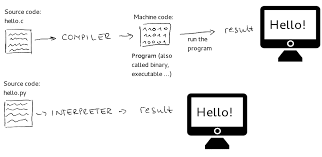
\includegraphics{index.png}
\caption{Interpreted vs compiled language}
\end{figure}

\hypertarget{which-python-should-i-use}{%
\subsection{Which Python should I use
?}\label{which-python-should-i-use}}

Python, as basically all programs, comes in different version and
flavours.

The latest version is \(\tt{3.7}\) (but it is continously evolving),
however you'll see older versions floating around (e.g. \(\tt{2.7}\)).
This is because there are some big differences between
\(\tt{Python 2.X}\) and \(\tt{Python 3.X}\) which prevent a sizeable
portion of \(\tt{Python 2}\) users to stick with it (moving to
\(\tt{Python 3}\) would require sizeable amount of work for big
projects).

\textbf{We will go for \(\tt{Python 3.X}\) anyway !}

Any Python interpreter, available at http://www.python.org, comes with a
standard set of \emph{packages} (will see in a while what they are), but
if you want more functionality, you can download more of them (there are
zillions of packages out there).

Some examples are:

\begin{itemize}
\tightlist
\item
  Numpy - which provides matrix algebra functionality;
\item
  Scipy - which provides a whole series of scientific computing
  functions;
\item
  Pandas - which provides tools for manipulating time series or dataset
  in general;
\item
  Matplotlib - for plotting graphs;
\item
  Jupyter - for notebooks like this one;
\item
  \ldots{}and many more.
\end{itemize}

\hypertarget{how-can-i-use-python}{%
\subsection{How can I use Python ?}\label{how-can-i-use-python}}

Once you have downloaded a Python distribution, there are various ways
of actually using it.

\begin{itemize}
\tightlist
\item
  The most immediate way is to just execute \(\tt{python.exe}\) on the
  command line to get a Python console for interacting with the
  interpreter.
\item
  If you are learining Python or do some simple data analysis, Jupyter
  notebooks (i.e.~this document) allow to see the results of your code
  as you write it, as well as make notes, plot graphs and so on.
\item
  If you are a programmer and want to do more complex things, you'll
  usually want one or more scripts, perhaps linked together, and execute
  one of them again using \(\tt{python.exe}\). For this last case an
  integrated development environment (IDE) can be very useful. An IDE is
  a graphical user interface which makes writing complex code easier by
  providing a text editor, a file browser, a debugger (a tool that helps
  you to spot mistakes in your code) all in one software application.
  Good example is \(\tt{PyCharm}\) (https://www.jetbrains.com/pycharm/)
  or repl.it an online IDE.
\end{itemize}

\hypertarget{how-we-will-use-it}{%
\subsection{How we will use it}\label{how-we-will-use-it}}

To avoid time consuming installations we will mainly use online tools so
that all you need is just a browser (Firefox :-), Chrome :-), Explorer
:-(). For completeness from time to time I will show you code running in
in a more advanced IDE called \texttt{PyCharm} but you won't need to
install it. So our tool are:

\begin{itemize}
\tightlist
\item
  \texttt{repl.it}, an online IDE to develop the more complicated
  projects in these lessions;
\item
  \texttt{colab}, an online notebook editor from Google.
\end{itemize}

As you can imagine there are many more similar tools available which
have more or less the same functionality as the one proposed
(e.g.~cocalc a possible replacement of colab). Another possibility,
quite flexible but slightly more complicated to setup, is Anaconda
Python. It's free to download and works on Windows, Mac or Linux and has
been used in the past years for this course. Those interested can take a
look at https://www.anaconda.com.

\hypertarget{online-courses}{%
\subsection{Online courses}\label{online-courses}}

Python popularity is growing every day so it is very easy to find good
(and free) online courses looking in Google. Since in this course we do
not have time to cover in depth the potentiality of this language I
strongly suggest you to spend some time in watching one of them. One
example could be

\textbf{MITx: 6.00.1x Introduction to Computer Science and Programming
Using Python}
https://courses.edx.org/courses/course-v1:MITx+6.00.1x+2T2017\_2/course/

\hypertarget{lets-spend-few-minutes-all-together-to-setup-the-software}{%
\subsubsection{Let's spend few minutes all together to setup the
software}\label{lets-spend-few-minutes-all-together-to-setup-the-software}}

\hypertarget{python-basics}{%
\subsection{Python basics}\label{python-basics}}

Try the commands I will explain in the remaining part of the lession
either typing them in a \texttt{colab} notebook or using the interactive
shell of \texttt{repl.it}.

    \begin{Verbatim}[commandchars=\\\{\}]
{\color{incolor}In [{\color{incolor}1}]:} \PY{c+c1}{\PYZsh{} print is a keyword, reserved words that have a special meaning}
        \PY{n+nb}{print} \PY{p}{(}\PY{l+s+s2}{\PYZdq{}}\PY{l+s+s2}{Hello world !}\PY{l+s+s2}{\PYZdq{}}\PY{p}{)} 
\end{Verbatim}

    \begin{Verbatim}[commandchars=\\\{\}]
Hello world !

    \end{Verbatim}

    \begin{Verbatim}[commandchars=\\\{\}]
{\color{incolor}In [{\color{incolor}2}]:} \PY{n+nb}{print} \PY{p}{(}\PY{l+s+s2}{\PYZdq{}}\PY{l+s+s2}{Welcome}\PY{l+s+s2}{\PYZdq{}}\PY{p}{)}
        \PY{n+nb}{print} \PY{p}{(}\PY{l+s+s2}{\PYZdq{}}\PY{l+s+s2}{to}\PY{l+s+s2}{\PYZdq{}}\PY{p}{)}
        \PY{n+nb}{print} \PY{p}{(}\PY{l+s+s2}{\PYZdq{}}\PY{l+s+s2}{everybody}\PY{l+s+s2}{\PYZdq{}}\PY{p}{)}
\end{Verbatim}

    \begin{Verbatim}[commandchars=\\\{\}]
Welcome
to
everybody

    \end{Verbatim}

    \begin{Verbatim}[commandchars=\\\{\}]
{\color{incolor}In [{\color{incolor}3}]:} \PY{c+c1}{\PYZsh{} this is a comment and the next line prints \PYZdq{}Ciao\PYZdq{}}
        \PY{n+nb}{print} \PY{p}{(}\PY{l+s+s2}{\PYZdq{}}\PY{l+s+s2}{Ciao}\PY{l+s+s2}{\PYZdq{}}\PY{p}{)} \PY{c+c1}{\PYZsh{} comments like this are useful to explain what\PYZsq{}s going on in the }
                       \PY{c+c1}{\PYZsh{} code you write}
\end{Verbatim}

    \begin{Verbatim}[commandchars=\\\{\}]
Ciao

    \end{Verbatim}

    \hypertarget{exercise-1.1}{%
\subsubsection{Exercise 1.1}\label{exercise-1.1}}

Write few lines of code in your notebook or in the interactive shell
that print on the display ``Hello !''

\hypertarget{variables}{%
\subsection{Variables}\label{variables}}

Variables are used to store information to be referenced and manipulated
in a computer program (e.g.~a number, a string\ldots{}).

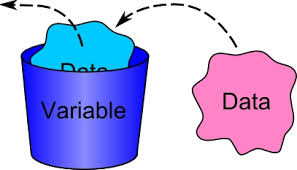
\includegraphics{var1.jpeg} 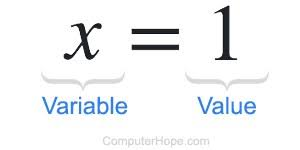
\includegraphics{var2.jpeg}

    \begin{Verbatim}[commandchars=\\\{\}]
{\color{incolor}In [{\color{incolor}4}]:} \PY{n}{x} \PY{o}{=} \PY{l+m+mi}{9} \PY{c+c1}{\PYZsh{} assign number 9 to variable named x}
\end{Verbatim}

    \begin{Verbatim}[commandchars=\\\{\}]
{\color{incolor}In [{\color{incolor}5}]:} \PY{n}{x} \PY{c+c1}{\PYZsh{} in console typing just a variable is equivalent to print its value}
\end{Verbatim}

\begin{Verbatim}[commandchars=\\\{\}]
{\color{outcolor}Out[{\color{outcolor}5}]:} 9
\end{Verbatim}
            
    \begin{Verbatim}[commandchars=\\\{\}]
{\color{incolor}In [{\color{incolor}6}]:} \PY{n}{myphone} \PY{o}{=} \PY{l+s+s2}{\PYZdq{}}\PY{l+s+s2}{Huawei P10Lite}\PY{l+s+s2}{\PYZdq{}}
\end{Verbatim}

    \begin{Verbatim}[commandchars=\\\{\}]
{\color{incolor}In [{\color{incolor}7}]:} \PY{n+nb}{print} \PY{p}{(}\PY{n}{myphone}\PY{p}{)}
\end{Verbatim}

    \begin{Verbatim}[commandchars=\\\{\}]
Huawei P10Lite

    \end{Verbatim}

    \begin{Verbatim}[commandchars=\\\{\}]
{\color{incolor}In [{\color{incolor}8}]:} \PY{n+nb}{print} \PY{p}{(}\PY{n+nb}{type}\PY{p}{(}\PY{n}{x}\PY{p}{)}\PY{p}{)}       \PY{c+c1}{\PYZsh{} the type keyword tells you which kind of object is }
                              \PY{c+c1}{\PYZsh{} stored in a variable}
        \PY{n+nb}{print} \PY{p}{(}\PY{n+nb}{type}\PY{p}{(}\PY{n}{myphone}\PY{p}{)}\PY{p}{)} \PY{c+c1}{\PYZsh{} int\PYZhy{}\PYZgt{}integer, str\PYZhy{}\PYZgt{}string we will see later in more}
                              \PY{c+c1}{\PYZsh{} detail what is a string}
\end{Verbatim}

    \begin{Verbatim}[commandchars=\\\{\}]
<class 'int'>
<class 'str'>

    \end{Verbatim}

    \hypertarget{python-variable-name-rules}{%
\subsubsection{Python variable name
rules}\label{python-variable-name-rules}}

A Python variable name must: * begin with a letter (myphone) or
underscore (\_myphone); * other characters can be letters, numbers or
more \_; * variable names are case-sensitive so myphone and myPhone are
two distinct variables;

\textbf{There are some reserved words which you cannot use as a variable
name because Python uses them for other things (e.g.
\(\tt{print, type, for...}\))}.

To use GOOD variable names always choose meaningful names instead of
short names (i.e. \(\tt{numberOfCakes}\) is much better than simply
\(\tt{n}\)), try to be consistent with your conventions (e.g.~choose
once and for all between \(\tt{number\_of\_cakes}\) or
\(\tt{numberofcakes}\) or \(\tt{numberOfCakes}\)), usually begin a
variable name with underscore (\_) only for a special case (will see
later when this is usually done).

\hypertarget{mathematical-expressions}{%
\subsection{Mathematical expressions}\label{mathematical-expressions}}

    \begin{Verbatim}[commandchars=\\\{\}]
{\color{incolor}In [{\color{incolor}9}]:} \PY{l+m+mi}{1} \PY{o}{+} \PY{l+m+mi}{2}
\end{Verbatim}

\begin{Verbatim}[commandchars=\\\{\}]
{\color{outcolor}Out[{\color{outcolor}9}]:} 3
\end{Verbatim}
            
    \begin{Verbatim}[commandchars=\\\{\}]
{\color{incolor}In [{\color{incolor}10}]:} \PY{l+m+mi}{40} \PY{o}{\PYZhy{}} \PY{l+m+mi}{5}
\end{Verbatim}

\begin{Verbatim}[commandchars=\\\{\}]
{\color{outcolor}Out[{\color{outcolor}10}]:} 35
\end{Verbatim}
            
    \begin{Verbatim}[commandchars=\\\{\}]
{\color{incolor}In [{\color{incolor}11}]:} \PY{n}{x} \PY{o}{*} \PY{l+m+mi}{20} \PY{c+c1}{\PYZsh{} remember that we set x equal to 9}
\end{Verbatim}

\begin{Verbatim}[commandchars=\\\{\}]
{\color{outcolor}Out[{\color{outcolor}11}]:} 180
\end{Verbatim}
            
    \begin{Verbatim}[commandchars=\\\{\}]
{\color{incolor}In [{\color{incolor}12}]:} \PY{n}{x} \PY{o}{/} \PY{l+m+mi}{4}
\end{Verbatim}

\begin{Verbatim}[commandchars=\\\{\}]
{\color{outcolor}Out[{\color{outcolor}12}]:} 2.25
\end{Verbatim}
            
    \begin{Verbatim}[commandchars=\\\{\}]
{\color{incolor}In [{\color{incolor}13}]:} \PY{n+nb}{print} \PY{p}{(}\PY{n+nb}{type}\PY{p}{(}\PY{l+m+mf}{2.25}\PY{p}{)}\PY{p}{)} \PY{c+c1}{\PYZsh{} this is a new type: floating\PYZhy{}point value}
\end{Verbatim}

    \begin{Verbatim}[commandchars=\\\{\}]
<class 'float'>

    \end{Verbatim}

    \begin{Verbatim}[commandchars=\\\{\}]
{\color{incolor}In [{\color{incolor}14}]:} \PY{n}{x} \PY{o}{/}\PY{o}{/} \PY{l+m+mi}{4} \PY{c+c1}{\PYZsh{} interger division \PYZhy{} result will be truncated to the }
                \PY{c+c1}{\PYZsh{} corresponding integer (no rounding)}
                \PY{c+c1}{\PYZsh{} 11 / 3 = 3.666666 \PYZhy{}\PYZgt{} 11 // 3 = 3}
\end{Verbatim}

\begin{Verbatim}[commandchars=\\\{\}]
{\color{outcolor}Out[{\color{outcolor}14}]:} 2
\end{Verbatim}
            
    \begin{Verbatim}[commandchars=\\\{\}]
{\color{incolor}In [{\color{incolor}15}]:} \PY{n}{y} \PY{o}{=} \PY{l+m+mi}{3}
         \PY{n}{x} \PY{o}{*}\PY{o}{*} \PY{n}{y} \PY{c+c1}{\PYZsh{} x to the power of y}
\end{Verbatim}

\begin{Verbatim}[commandchars=\\\{\}]
{\color{outcolor}Out[{\color{outcolor}15}]:} 729
\end{Verbatim}
            
    \begin{Verbatim}[commandchars=\\\{\}]
{\color{incolor}In [{\color{incolor}16}]:} \PY{l+m+mi}{3} \PY{o}{*} \PY{p}{(}\PY{n}{x} \PY{o}{+} \PY{n}{y}\PY{p}{)}
\end{Verbatim}

\begin{Verbatim}[commandchars=\\\{\}]
{\color{outcolor}Out[{\color{outcolor}16}]:} 36
\end{Verbatim}
            
    \begin{Verbatim}[commandchars=\\\{\}]
{\color{incolor}In [{\color{incolor}17}]:} \PY{n}{log}\PY{p}{(}\PY{l+m+mi}{3}\PY{p}{)} \PY{c+c1}{\PYZsh{} causes an error because the logarithm function }
                \PY{c+c1}{\PYZsh{} is not available by default}
\end{Verbatim}

    \begin{Verbatim}[commandchars=\\\{\}]

        ---------------------------------------------------------------------------

        NameError                                 Traceback (most recent call last)

        <ipython-input-17-ffde4d60496a> in <module>()
    ----> 1 log(3) \# causes an error because the logarithm function
          2        \# is not available by default


        NameError: name 'log' is not defined

    \end{Verbatim}

    \hypertarget{modules}{%
\subsection{Modules}\label{modules}}

Useful functions can be saved in libraries (called \emph{modules}) so
that thay can be re-used in different programs. The keyword
\emph{import} allows to load functions and data from other Python files
(\emph{modules}) and make them available in your program. Python already
comes with a lot of built-in modules for doing lots of different tasks
(the so called \emph{standard library}) but many more modules are
available for download on the web and you can of course write your own !

\begin{figure}
\centering
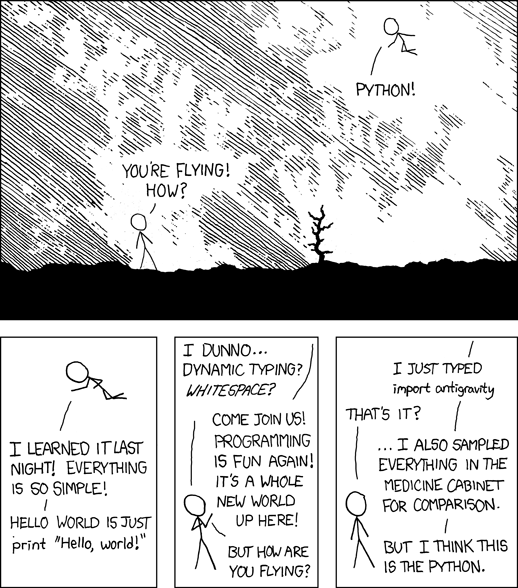
\includegraphics{python.png}
\caption{Python has many modules for download on the web\ldots{}}
\end{figure}

    \begin{Verbatim}[commandchars=\\\{\}]
{\color{incolor}In [{\color{incolor}18}]:} \PY{k+kn}{import} \PY{n+nn}{math}
         \PY{n+nb}{dir}\PY{p}{(}\PY{n}{math}\PY{p}{)} \PY{c+c1}{\PYZsh{} dir keyword lists the content of a module}
\end{Verbatim}

\begin{Verbatim}[commandchars=\\\{\}]
{\color{outcolor}Out[{\color{outcolor}18}]:} ['\_\_doc\_\_',
          '\_\_loader\_\_',
          '\_\_name\_\_',
          '\_\_package\_\_',
          '\_\_spec\_\_',
          'acos',
          'acosh',
          'asin',
          'asinh',
          'atan',
          'atan2',
          'atanh',
          'ceil',
          'copysign',
          'cos',
          'cosh',
          'degrees',
          'e',
          'erf',
          'erfc',
          'exp',
          'expm1',
          'fabs',
          'factorial',
          'floor',
          'fmod',
          'frexp',
          'fsum',
          'gamma',
          'gcd',
          'hypot',
          'inf',
          'isclose',
          'isfinite',
          'isinf',
          'isnan',
          'ldexp',
          'lgamma',
          'log',
          'log10',
          'log1p',
          'log2',
          'modf',
          'nan',
          'pi',
          'pow',
          'radians',
          'remainder',
          'sin',
          'sinh',
          'sqrt',
          'tan',
          'tanh',
          'tau',
          'trunc']
\end{Verbatim}
            
    \textbf{Once a module has been imported, the functions it contains can
be accessed with a \emph{dot} ``module\_name.function\_name'':}

    \begin{Verbatim}[commandchars=\\\{\}]
{\color{incolor}In [{\color{incolor}19}]:} \PY{n}{math}\PY{o}{.}\PY{n}{log}\PY{p}{(}\PY{l+m+mi}{3}\PY{p}{)}
\end{Verbatim}

\begin{Verbatim}[commandchars=\\\{\}]
{\color{outcolor}Out[{\color{outcolor}19}]:} 1.0986122886681098
\end{Verbatim}
            
    \begin{Verbatim}[commandchars=\\\{\}]
{\color{incolor}In [{\color{incolor}20}]:} \PY{n}{math}\PY{o}{.}\PY{n}{exp}\PY{p}{(}\PY{l+m+mi}{3}\PY{p}{)}
\end{Verbatim}

\begin{Verbatim}[commandchars=\\\{\}]
{\color{outcolor}Out[{\color{outcolor}20}]:} 20.085536923187668
\end{Verbatim}
            
    \begin{Verbatim}[commandchars=\\\{\}]
{\color{incolor}In [{\color{incolor}21}]:} \PY{n+nb}{print} \PY{p}{(}\PY{n+nb}{type}\PY{p}{(}\PY{n}{math}\PY{o}{.}\PY{n}{log}\PY{p}{)}\PY{p}{)} \PY{c+c1}{\PYZsh{} yet another type: builtin function}
         \PY{n+nb}{print} \PY{p}{(}\PY{n+nb}{type}\PY{p}{(}\PY{n}{math}\PY{o}{.}\PY{n}{log}\PY{p}{(}\PY{l+m+mi}{3}\PY{p}{)}\PY{p}{)}\PY{p}{)}
\end{Verbatim}

    \begin{Verbatim}[commandchars=\\\{\}]
<class 'builtin\_function\_or\_method'>
<class 'float'>

    \end{Verbatim}

    Since we are lazy and we don't want to type ``math.'' every time we
compute a logarithm or an exponential, we can use the following syntax:

    \begin{Verbatim}[commandchars=\\\{\}]
{\color{incolor}In [{\color{incolor}22}]:} \PY{k+kn}{from} \PY{n+nn}{math} \PY{k}{import} \PY{n}{log}\PY{p}{,} \PY{n}{exp}
         \PY{n+nb}{print} \PY{p}{(}\PY{n}{log}\PY{p}{(}\PY{l+m+mi}{3}\PY{p}{)}\PY{p}{)}
         \PY{n+nb}{print} \PY{p}{(}\PY{n}{exp}\PY{p}{(}\PY{l+m+mi}{3}\PY{p}{)}\PY{p}{)}
\end{Verbatim}

    \begin{Verbatim}[commandchars=\\\{\}]
1.0986122886681098
20.085536923187668

    \end{Verbatim}

    Putting together what we have learned so far we can try to save the
result of an expression in a variable (or even in the same variable we
started with). As an example let's compute the interest rate \(r\) that
produces a return \(R\) of about 1051.71 Euro when investing 10000 Euro
for 2 years:

\(R = N\mathrm{e}^{r\tau} \rightarrow r = \frac{1}{\tau} \mathrm{log}(\frac{R}{N})\)

    \begin{Verbatim}[commandchars=\\\{\}]
{\color{incolor}In [{\color{incolor}23}]:} \PY{n}{rate} \PY{o}{=} \PY{p}{(}\PY{l+m+mi}{1}\PY{o}{/}\PY{l+m+mi}{2}\PY{p}{)}\PY{o}{*}\PY{n}{log}\PY{p}{(}\PY{l+m+mf}{11051.71}\PY{o}{/}\PY{l+m+mi}{10000}\PY{p}{)}
         \PY{n+nb}{print} \PY{p}{(}\PY{n}{rate}\PY{p}{)}
         \PY{n}{x} \PY{o}{=} \PY{n}{x} \PY{o}{+} \PY{l+m+mi}{1}    \PY{c+c1}{\PYZsh{} the value of x was 9 when was used last}
         \PY{n}{x} \PY{o}{+}\PY{o}{=} \PY{l+m+mi}{1}       \PY{c+c1}{\PYZsh{} += is a shortcut for x = x + 1}
         \PY{n+nb}{print} \PY{p}{(}\PY{n}{x}\PY{p}{)}
\end{Verbatim}

    \begin{Verbatim}[commandchars=\\\{\}]
0.05000003706410832
11

    \end{Verbatim}

    \hypertarget{exercise-1.2}{%
\subsubsection{Exercise 1.2}\label{exercise-1.2}}

Write code in your notebook or in the interactive shell to print the
natural logarithm of your year of birth (expected something like:
7.587817219993427)

\hypertarget{boolean-expressions}{%
\subsection{Boolean expressions}\label{boolean-expressions}}

The expressions we have seen so far evaluate to a number. Boolean
expressions evaluate to \(\tt{true}\) or \(\tt{false}\). Sometimes they
involves logical or comparison operators like \(\tt{or}\), \(\tt{and}\),
\textgreater{} (greater than), \textless{} (less than)\ldots{} Let's see
some example.

    \begin{Verbatim}[commandchars=\\\{\}]
{\color{incolor}In [{\color{incolor}24}]:} \PY{l+m+mi}{1} \PY{o}{==} \PY{l+m+mi}{2} 
         \PY{c+c1}{\PYZsh{} single = assigns a value to a variable like in x = 9}
         \PY{c+c1}{\PYZsh{} double == checks the equality of two objects}
\end{Verbatim}

\begin{Verbatim}[commandchars=\\\{\}]
{\color{outcolor}Out[{\color{outcolor}24}]:} False
\end{Verbatim}
            
    \begin{Verbatim}[commandchars=\\\{\}]
{\color{incolor}In [{\color{incolor}25}]:} \PY{l+m+mi}{1} \PY{o}{!=} \PY{l+m+mi}{2} \PY{c+c1}{\PYZsh{} != is the \PYZdq{}not equal to\PYZdq{} operator}
\end{Verbatim}

\begin{Verbatim}[commandchars=\\\{\}]
{\color{outcolor}Out[{\color{outcolor}25}]:} True
\end{Verbatim}
            
    \begin{Verbatim}[commandchars=\\\{\}]
{\color{incolor}In [{\color{incolor}26}]:} \PY{l+m+mi}{2} \PY{o}{\PYZlt{}} \PY{l+m+mi}{2}
\end{Verbatim}

\begin{Verbatim}[commandchars=\\\{\}]
{\color{outcolor}Out[{\color{outcolor}26}]:} False
\end{Verbatim}
            
    \begin{Verbatim}[commandchars=\\\{\}]
{\color{incolor}In [{\color{incolor}27}]:} \PY{l+m+mi}{2} \PY{o}{\PYZlt{}}\PY{o}{=} \PY{l+m+mi}{2}  \PY{c+c1}{\PYZsh{} in this case we allow the numbers to be equal too}
\end{Verbatim}

\begin{Verbatim}[commandchars=\\\{\}]
{\color{outcolor}Out[{\color{outcolor}27}]:} True
\end{Verbatim}
            
    \begin{Verbatim}[commandchars=\\\{\}]
{\color{incolor}In [{\color{incolor}28}]:} \PY{n+nb}{print} \PY{p}{(}\PY{n}{x}\PY{p}{)}
         \PY{l+m+mi}{15} \PY{o}{\PYZlt{}}\PY{o}{=} \PY{n}{x} \PY{o+ow}{and} \PY{n}{x} \PY{o}{\PYZlt{}}\PY{o}{=} \PY{l+m+mi}{20} \PY{c+c1}{\PYZsh{} this expression could also be written as 15 \PYZlt{}= x \PYZlt{}= 20}
\end{Verbatim}

    \begin{Verbatim}[commandchars=\\\{\}]
11

    \end{Verbatim}

\begin{Verbatim}[commandchars=\\\{\}]
{\color{outcolor}Out[{\color{outcolor}28}]:} False
\end{Verbatim}
            
    \begin{Verbatim}[commandchars=\\\{\}]
{\color{incolor}In [{\color{incolor}29}]:} \PY{l+m+mi}{15} \PY{o}{\PYZlt{}}\PY{o}{=} \PY{n}{x} \PY{o+ow}{or} \PY{n}{x} \PY{o}{\PYZlt{}}\PY{o}{=} \PY{l+m+mi}{20}
\end{Verbatim}

\begin{Verbatim}[commandchars=\\\{\}]
{\color{outcolor}Out[{\color{outcolor}29}]:} True
\end{Verbatim}
            
    \begin{Verbatim}[commandchars=\\\{\}]
{\color{incolor}In [{\color{incolor}30}]:} \PY{o+ow}{not} \PY{p}{(}\PY{n}{x} \PY{o}{\PYZgt{}} \PY{l+m+mi}{20}\PY{p}{)} \PY{c+c1}{\PYZsh{} the not keyword negates the following expression}
\end{Verbatim}

\begin{Verbatim}[commandchars=\\\{\}]
{\color{outcolor}Out[{\color{outcolor}30}]:} True
\end{Verbatim}
            
    \hypertarget{string-expressions}{%
\subsection{String expressions}\label{string-expressions}}

A ``string'' is a sequence of characters (letters, digits, spaces,
punctiation, new lines\ldots{})

    \begin{Verbatim}[commandchars=\\\{\}]
{\color{incolor}In [{\color{incolor}31}]:} \PY{n}{mystring} \PY{o}{=} \PY{l+s+s2}{\PYZdq{}}\PY{l+s+s2}{some text with punctuation, spaces and digits 10}\PY{l+s+s2}{\PYZdq{}}
\end{Verbatim}

    \begin{Verbatim}[commandchars=\\\{\}]
{\color{incolor}In [{\color{incolor}32}]:} \PY{l+s+s2}{\PYZdq{}}\PY{l+s+s2}{abc}\PY{l+s+s2}{\PYZdq{}} \PY{o}{+} \PY{l+s+s2}{\PYZdq{}}\PY{l+s+s2}{def}\PY{l+s+s2}{\PYZdq{}} \PY{c+c1}{\PYZsh{} it is possible to concatenate strings with + }
\end{Verbatim}

\begin{Verbatim}[commandchars=\\\{\}]
{\color{outcolor}Out[{\color{outcolor}32}]:} 'abcdef'
\end{Verbatim}
            
    \begin{Verbatim}[commandchars=\\\{\}]
{\color{incolor}In [{\color{incolor}33}]:} \PY{l+s+s2}{\PYZdq{}}\PY{l+s+s2}{The number }\PY{l+s+s2}{\PYZdq{}} \PY{o}{+} \PY{l+m+mi}{4} \PY{o}{+} \PY{l+s+s2}{\PYZdq{}}\PY{l+s+s2}{ is my favourite number}\PY{l+s+s2}{\PYZdq{}}
         \PY{c+c1}{\PYZsh{} this causes an error since we are trying to concatenate a string }
         \PY{c+c1}{\PYZsh{} with a number so two different kind of objects}
\end{Verbatim}

    \begin{Verbatim}[commandchars=\\\{\}]

        ---------------------------------------------------------------------------

        TypeError                                 Traceback (most recent call last)

        <ipython-input-33-b9f65c5a45f7> in <module>()
    ----> 1 "The number " + 4 + " is my favourite number"
          2 \# this causes an error since we are trying to concatenate a string
          3 \# with a number so two different kind of objects


        TypeError: can only concatenate str (not "int") to str

    \end{Verbatim}

    To avoid this error is possible to \emph{cast} an object to a different
type, Python will try then to convert it to the desired type. This is
not always possible though: for example a number can be converted to a
string (e.g.~from the integer 4 to the actual symbol ``4'') but the
opposite is not possible (e.g.~cannot convert the string ``matteo'' to a
meaningful number)

    \begin{Verbatim}[commandchars=\\\{\}]
{\color{incolor}In [{\color{incolor}34}]:} \PY{l+s+s2}{\PYZdq{}}\PY{l+s+s2}{The number }\PY{l+s+s2}{\PYZdq{}} \PY{o}{+} \PY{n+nb}{str}\PY{p}{(}\PY{l+m+mi}{4}\PY{p}{)} \PY{o}{+} \PY{l+s+s2}{\PYZdq{}}\PY{l+s+s2}{ is my favourite number}\PY{l+s+s2}{\PYZdq{}} \PY{c+c1}{\PYZsh{} str() cast the number to a string}
\end{Verbatim}

\begin{Verbatim}[commandchars=\\\{\}]
{\color{outcolor}Out[{\color{outcolor}34}]:} 'The number 4 is my favourite number'
\end{Verbatim}
            
    \begin{Verbatim}[commandchars=\\\{\}]
{\color{incolor}In [{\color{incolor}35}]:} \PY{n+nb}{print} \PY{p}{(}\PY{n+nb}{type}\PY{p}{(}\PY{l+m+mf}{3.4}\PY{p}{)}\PY{p}{)}
         \PY{n+nb}{print} \PY{p}{(}\PY{n+nb}{type}\PY{p}{(}\PY{n+nb}{str}\PY{p}{(}\PY{l+m+mf}{3.4}\PY{p}{)}\PY{p}{)}\PY{p}{)}
\end{Verbatim}

    \begin{Verbatim}[commandchars=\\\{\}]
<class 'float'>
<class 'str'>

    \end{Verbatim}

    Instead of using + to concatenate strings, Python allows for a prettier
formatting using the following syntax (which for example allows for
float rounding):

    \begin{Verbatim}[commandchars=\\\{\}]
{\color{incolor}In [{\color{incolor}36}]:} \PY{l+s+s2}{\PYZdq{}}\PY{l+s+s2}{The speed of light is about }\PY{l+s+si}{\PYZob{}:.1f\PYZcb{}}\PY{l+s+s2}{ }\PY{l+s+si}{\PYZob{}\PYZcb{}}\PY{l+s+s2}{\PYZdq{}}\PY{o}{.}\PY{n}{format}\PY{p}{(}\PY{l+m+mf}{299792.458}\PY{p}{,} \PY{l+s+s2}{\PYZdq{}}\PY{l+s+s2}{km/s}\PY{l+s+s2}{\PYZdq{}}\PY{p}{)}
         \PY{c+c1}{\PYZsh{} each \PYZob{}\PYZcb{} is mapped to the variables listed later in the \PYZdq{}format\PYZdq{}}
\end{Verbatim}

\begin{Verbatim}[commandchars=\\\{\}]
{\color{outcolor}Out[{\color{outcolor}36}]:} 'The speed of light is about 299792.5 km/s'
\end{Verbatim}
            
    \hypertarget{indented-blocks-and-the-ttifelse-statement}{%
\subsection{\texorpdfstring{Indented blocks and the \(\tt{if/else}\)
statement}{Indented blocks and the \textbackslash{}tt\{if/else\} statement}}\label{indented-blocks-and-the-ttifelse-statement}}

Unlike other languages which uses parenthesis to isolate blocks of code
Python uses indentation. A first example of this is given by the
\(\tt{if/then}\) statements where based on some condition we can run
different part of the code.

    \begin{Verbatim}[commandchars=\\\{\}]
{\color{incolor}In [{\color{incolor}37}]:} \PY{c+c1}{\PYZsh{} remember x value is 13 now}
         \PY{k}{if} \PY{n}{x} \PY{o}{==} \PY{l+m+mi}{1}\PY{p}{:} 
             \PY{n+nb}{print} \PY{p}{(}\PY{l+s+s2}{\PYZdq{}}\PY{l+s+s2}{This will not be printed}\PY{l+s+s2}{\PYZdq{}}\PY{p}{)} 
             \PY{c+c1}{\PYZsh{} the block of code that is run if the first condition is met is indented}
         \PY{k}{elif} \PY{n}{x} \PY{o}{==} \PY{l+m+mi}{15}\PY{p}{:}
             \PY{n+nb}{print} \PY{p}{(}\PY{l+s+s2}{\PYZdq{}}\PY{l+s+s2}{This will not be printed either}\PY{l+s+s2}{\PYZdq{}}\PY{p}{)}
             \PY{c+c1}{\PYZsh{} again the block of code that is run here is indented to be \PYZdq{}isolated\PYZdq{} by the rest }
         \PY{k}{else}\PY{p}{:}
             \PY{n+nb}{print} \PY{p}{(}\PY{l+s+s2}{\PYZdq{}}\PY{l+s+s2}{This *will* be printed}\PY{l+s+s2}{\PYZdq{}}\PY{p}{)}
\end{Verbatim}

    \begin{Verbatim}[commandchars=\\\{\}]
This *will* be printed

    \end{Verbatim}

    \begin{Verbatim}[commandchars=\\\{\}]
{\color{incolor}In [{\color{incolor}38}]:} \PY{c+c1}{\PYZsh{} if by mistake I forget to indent some block I get an error}
         \PY{k}{if} \PY{n}{x} \PY{o}{==} \PY{l+m+mi}{1}\PY{p}{:} 
         \PY{n+nb}{print} \PY{p}{(}\PY{l+s+s2}{\PYZdq{}}\PY{l+s+s2}{This will not be printed}\PY{l+s+s2}{\PYZdq{}}\PY{p}{)}
         \PY{k}{elif} \PY{n}{x} \PY{o}{==} \PY{l+m+mi}{15}\PY{p}{:}
             \PY{n+nb}{print} \PY{p}{(}\PY{l+s+s2}{\PYZdq{}}\PY{l+s+s2}{This will not be printed either}\PY{l+s+s2}{\PYZdq{}}\PY{p}{)}
         \PY{k}{else}\PY{p}{:}
             \PY{n+nb}{print} \PY{p}{(}\PY{l+s+s2}{\PYZdq{}}\PY{l+s+s2}{This *will* be printed}\PY{l+s+s2}{\PYZdq{}}\PY{p}{)}
\end{Verbatim}

    \begin{Verbatim}[commandchars=\\\{\}]

          File "<ipython-input-38-4535a45a6419>", line 3
        print ("This will not be printed")
            \^{}
    IndentationError: expected an indented block


    \end{Verbatim}

    \begin{Verbatim}[commandchars=\\\{\}]
{\color{incolor}In [{\color{incolor}39}]:} \PY{k}{if} \PY{n}{x} \PY{o}{!=} \PY{l+m+mi}{1}\PY{p}{:}
             \PY{n+nb}{print} \PY{p}{(}\PY{l+s+s2}{\PYZdq{}}\PY{l+s+s2}{x does not equal to 1}\PY{l+s+s2}{\PYZdq{}}\PY{p}{)}
\end{Verbatim}

    \begin{Verbatim}[commandchars=\\\{\}]
x does not equal to 1

    \end{Verbatim}

    As an example, in C++ the previous code would have been:

\begin{Shaded}
\begin{Highlighting}[]
\ControlFlowTok{if}\NormalTok{ (x == }\DecValTok{1}\NormalTok{) \{}
\NormalTok{ print (}\StringTok{"This will not be printed"}\NormalTok{);}
\NormalTok{\}}
\ControlFlowTok{else} \ControlFlowTok{if}\NormalTok{ (x == }\DecValTok{15}\NormalTok{) \{}
\NormalTok{  print (}\StringTok{"This will not be printed either"}\NormalTok{);}
\NormalTok{\}}
\ControlFlowTok{else}\NormalTok{ \{}
\NormalTok{print (}\StringTok{"This *will* be printed"}\NormalTok{);}
\NormalTok{\}}
\end{Highlighting}
\end{Shaded}

N.B. Notice how indentation doesn't matter at all here.

\hypertarget{loops}{%
\subsection{Loops}\label{loops}}

Another very import feature of a language is the loop that allows to
repeat the same block of code many times. In Python loops can be coded
with \(\tt{for}\) or \(\tt{while}\) keywords.

\hypertarget{for}{%
\subsubsection{for}\label{for}}

    \begin{Verbatim}[commandchars=\\\{\}]
{\color{incolor}In [{\color{incolor}40}]:} \PY{c+c1}{\PYZsh{} the range keyword returns a \PYZdq{}list\PYZdq{} of integers starting from 0}
         \PY{k}{for} \PY{n}{i} \PY{o+ow}{in} \PY{n+nb}{range}\PY{p}{(}\PY{l+m+mi}{5}\PY{p}{)}\PY{p}{:}
             \PY{n+nb}{print} \PY{p}{(}\PY{n}{i}\PY{p}{)}
\end{Verbatim}

    \begin{Verbatim}[commandchars=\\\{\}]
0
1
2
3
4

    \end{Verbatim}

    \begin{Verbatim}[commandchars=\\\{\}]
{\color{incolor}In [{\color{incolor}41}]:} \PY{k}{for} \PY{n}{i} \PY{o+ow}{in} \PY{n+nb}{range}\PY{p}{(}\PY{l+m+mi}{25}\PY{p}{,} \PY{l+m+mi}{30}\PY{p}{)}\PY{p}{:} \PY{c+c1}{\PYZsh{} here both boundaries are specified}
             \PY{n+nb}{print} \PY{p}{(}\PY{n}{i}\PY{p}{)}
\end{Verbatim}

    \begin{Verbatim}[commandchars=\\\{\}]
25
26
27
28
29

    \end{Verbatim}

    \begin{Verbatim}[commandchars=\\\{\}]
{\color{incolor}In [{\color{incolor}42}]:} \PY{k}{for} \PY{n}{i} \PY{o+ow}{in} \PY{n+nb}{range} \PY{p}{(}\PY{l+m+mi}{30}\PY{p}{,} \PY{l+m+mi}{25}\PY{p}{,} \PY{o}{\PYZhy{}}\PY{l+m+mi}{1}\PY{p}{)}\PY{p}{:} \PY{c+c1}{\PYZsh{} here both boundaries and step are specified}
             \PY{n+nb}{print} \PY{p}{(}\PY{n}{i}\PY{p}{)}
\end{Verbatim}

    \begin{Verbatim}[commandchars=\\\{\}]
30
29
28
27
26

    \end{Verbatim}

    \begin{Verbatim}[commandchars=\\\{\}]
{\color{incolor}In [{\color{incolor}43}]:} \PY{k}{for} \PY{n}{i} \PY{o+ow}{in} \PY{n+nb}{range}\PY{p}{(}\PY{l+m+mi}{10}\PY{p}{)}\PY{p}{:}
             \PY{k}{if} \PY{n}{i} \PY{o}{==} \PY{l+m+mi}{5}\PY{p}{:}
                 \PY{k}{continue} \PY{c+c1}{\PYZsh{} this line skips the current iteration, }
                          \PY{c+c1}{\PYZsh{} 5 is actually missing from the output below}
             \PY{n+nb}{print} \PY{p}{(}\PY{n}{i}\PY{p}{)}
\end{Verbatim}

    \begin{Verbatim}[commandchars=\\\{\}]
0
1
2
3
4
6
7
8
9

    \end{Verbatim}

    \begin{Verbatim}[commandchars=\\\{\}]
{\color{incolor}In [{\color{incolor}44}]:} \PY{k}{for} \PY{n}{i} \PY{o+ow}{in} \PY{p}{(}\PY{l+m+mi}{4}\PY{p}{,} \PY{l+m+mi}{6}\PY{p}{,} \PY{l+m+mi}{10}\PY{p}{,} \PY{l+m+mi}{20}\PY{p}{)}\PY{p}{:} \PY{c+c1}{\PYZsh{} here we loop directly on a list of numbers}
             \PY{n+nb}{print} \PY{p}{(}\PY{n}{i}\PY{p}{)}
\end{Verbatim}

    \begin{Verbatim}[commandchars=\\\{\}]
4
6
10
20

    \end{Verbatim}

    \begin{Verbatim}[commandchars=\\\{\}]
{\color{incolor}In [{\color{incolor}45}]:} \PY{n}{phrase} \PY{o}{=} \PY{l+s+s1}{\PYZsq{}}\PY{l+s+s1}{how to loop over a string}\PY{l+s+s1}{\PYZsq{}}
         \PY{k}{for} \PY{n}{c} \PY{o+ow}{in} \PY{n}{phrase}\PY{p}{:}
             \PY{n+nb}{print} \PY{p}{(}\PY{n}{c}\PY{p}{)}
\end{Verbatim}

    \begin{Verbatim}[commandchars=\\\{\}]
h
o
w
 
t
o
 
l
o
o
p
 
o
v
e
r
 
a
 
s
t
r
i
n
g

    \end{Verbatim}

    \hypertarget{while}{%
\subsubsection{while}\label{while}}

In a for loop we go through all the elements of a list of objects, the
\texttt{while} statement instead repeats the same block of code untill a
condition is met.

    \begin{Verbatim}[commandchars=\\\{\}]
{\color{incolor}In [{\color{incolor}46}]:} \PY{n}{x} \PY{o}{=} \PY{l+m+mi}{1}
         \PY{k}{while} \PY{n}{x} \PY{o}{*}\PY{o}{*} \PY{l+m+mi}{2} \PY{o}{\PYZlt{}} \PY{l+m+mi}{50}\PY{p}{:} \PY{c+c1}{\PYZsh{} the following block of code is run if x squared is \PYZlt{}50}
             \PY{n+nb}{print} \PY{p}{(}\PY{n}{x}\PY{p}{)}
             \PY{n}{x} \PY{o}{+}\PY{o}{=} \PY{l+m+mi}{1} \PY{c+c1}{\PYZsh{} each time we increment by 1 the variable x}
\end{Verbatim}

    \begin{Verbatim}[commandchars=\\\{\}]
1
2
3
4
5
6
7

    \end{Verbatim}

    It is possible to exit prematurely from a while loop using the
\(\tt{break}\) keyword.

    \begin{Verbatim}[commandchars=\\\{\}]
{\color{incolor}In [{\color{incolor}47}]:} \PY{n}{x} \PY{o}{=} \PY{l+m+mi}{1}
         \PY{k}{while} \PY{k+kc}{True}\PY{p}{:} \PY{c+c1}{\PYZsh{} True is always true :\PYZhy{}) so this would run forever}
             \PY{k}{if} \PY{p}{(}\PY{n}{x} \PY{o}{*}\PY{o}{*} \PY{l+m+mi}{2} \PY{o}{\PYZgt{}} \PY{l+m+mi}{50}\PY{p}{)}\PY{p}{:} 
                 \PY{k}{break} \PY{c+c1}{\PYZsh{} this line exit from the while loop}
             \PY{n+nb}{print} \PY{p}{(}\PY{n}{x}\PY{p}{)}
             \PY{n}{x} \PY{o}{+}\PY{o}{=} \PY{l+m+mi}{1} 
\end{Verbatim}

    \begin{Verbatim}[commandchars=\\\{\}]
1
2
3
4
5
6
7

    \end{Verbatim}

    \hypertarget{lists}{%
\subsection{Lists}\label{lists}}

A list in Python is a container that is a \emph{mutable}, ordered
sequence of elements. Each element or value that is inside of a list is
called an item. Each item can be accessed using squared brackets (list
indexing is zero-based). It is considered mutable since you can add,
remove or update the items in the list. Ordered instead means that items
are kept in the same order they have been added to the list.

    \begin{Verbatim}[commandchars=\\\{\}]
{\color{incolor}In [{\color{incolor}48}]:} \PY{n}{mylist} \PY{o}{=} \PY{p}{[}\PY{l+m+mi}{21}\PY{p}{,} \PY{l+m+mi}{32}\PY{p}{,} \PY{l+m+mi}{15}\PY{p}{]}
         \PY{n}{mylist}
\end{Verbatim}

\begin{Verbatim}[commandchars=\\\{\}]
{\color{outcolor}Out[{\color{outcolor}48}]:} [21, 32, 15]
\end{Verbatim}
            
    \begin{Verbatim}[commandchars=\\\{\}]
{\color{incolor}In [{\color{incolor}49}]:} \PY{n+nb}{print} \PY{p}{(}\PY{n+nb}{type}\PY{p}{(}\PY{n}{mylist}\PY{p}{)}\PY{p}{)}
\end{Verbatim}

    \begin{Verbatim}[commandchars=\\\{\}]
<class 'list'>

    \end{Verbatim}

    \begin{Verbatim}[commandchars=\\\{\}]
{\color{incolor}In [{\color{incolor}50}]:} \PY{k}{for} \PY{n}{i} \PY{o+ow}{in} \PY{n+nb}{range}\PY{p}{(}\PY{n+nb}{len}\PY{p}{(}\PY{n}{mylist}\PY{p}{)}\PY{p}{)}\PY{p}{:} \PY{c+c1}{\PYZsh{} len() returns the number of items in a list}
             \PY{n+nb}{print} \PY{p}{(}\PY{n}{mylist}\PY{p}{[}\PY{n}{i}\PY{p}{]}\PY{p}{)}
\end{Verbatim}

    \begin{Verbatim}[commandchars=\\\{\}]
21
32
15

    \end{Verbatim}

    \begin{Verbatim}[commandchars=\\\{\}]
{\color{incolor}In [{\color{incolor}51}]:} \PY{n+nb}{len}\PY{p}{(}\PY{n}{mylist}\PY{p}{)}
\end{Verbatim}

\begin{Verbatim}[commandchars=\\\{\}]
{\color{outcolor}Out[{\color{outcolor}51}]:} 3
\end{Verbatim}
            
    \begin{Verbatim}[commandchars=\\\{\}]
{\color{incolor}In [{\color{incolor}52}]:} \PY{n}{mylist}\PY{p}{[}\PY{l+m+mi}{0}\PY{p}{]} \PY{c+c1}{\PYZsh{} accessing an item by index,remember the first item is element 0}
\end{Verbatim}

\begin{Verbatim}[commandchars=\\\{\}]
{\color{outcolor}Out[{\color{outcolor}52}]:} 21
\end{Verbatim}
            
    \begin{Verbatim}[commandchars=\\\{\}]
{\color{incolor}In [{\color{incolor}53}]:} \PY{n}{mylist}\PY{p}{[}\PY{l+m+mi}{1}\PY{p}{]} \PY{o}{=} \PY{l+m+mi}{74} \PY{c+c1}{\PYZsh{} we can change list items since it\PYZsq{}s *mutable*}
         \PY{n}{mylist}
\end{Verbatim}

\begin{Verbatim}[commandchars=\\\{\}]
{\color{outcolor}Out[{\color{outcolor}53}]:} [21, 74, 15]
\end{Verbatim}
            
    \begin{Verbatim}[commandchars=\\\{\}]
{\color{incolor}In [{\color{incolor}54}]:} \PY{n}{mylist}\PY{p}{[}\PY{l+m+mi}{3}\PY{p}{]} \PY{c+c1}{\PYZsh{} error ! it doesn\PYZsq{}t exists, the list has only 3 }
                   \PY{c+c1}{\PYZsh{} elements, so the last is item 2}
\end{Verbatim}

    \begin{Verbatim}[commandchars=\\\{\}]

        ---------------------------------------------------------------------------

        IndexError                                Traceback (most recent call last)

        <ipython-input-54-3a32eb4a7169> in <module>()
    ----> 1 mylist[3] \# error ! it doesn't exists, the list has only 3
          2           \# elements, so the last is item 2


        IndexError: list index out of range

    \end{Verbatim}

    \begin{Verbatim}[commandchars=\\\{\}]
{\color{incolor}In [{\color{incolor}55}]:} \PY{n}{mylist}\PY{p}{[}\PY{o}{\PYZhy{}}\PY{l+m+mi}{1}\PY{p}{]} \PY{c+c1}{\PYZsh{} negative index starts from the last element}
\end{Verbatim}

\begin{Verbatim}[commandchars=\\\{\}]
{\color{outcolor}Out[{\color{outcolor}55}]:} 15
\end{Verbatim}
            
    \begin{Verbatim}[commandchars=\\\{\}]
{\color{incolor}In [{\color{incolor}56}]:} \PY{n}{mylist}\PY{p}{[}\PY{l+m+mi}{1}\PY{p}{:}\PY{p}{]} \PY{c+c1}{\PYZsh{} : is called slice, all items starting from the second }
                    \PY{c+c1}{\PYZsh{} (remember indexing starts from 0)}
\end{Verbatim}

\begin{Verbatim}[commandchars=\\\{\}]
{\color{outcolor}Out[{\color{outcolor}56}]:} [74, 15]
\end{Verbatim}
            
    \begin{Verbatim}[commandchars=\\\{\}]
{\color{incolor}In [{\color{incolor}57}]:} \PY{n}{mylist}\PY{p}{[}\PY{p}{:}\PY{l+m+mi}{2}\PY{p}{]} \PY{c+c1}{\PYZsh{} elements up to but excluding item 2}
\end{Verbatim}

\begin{Verbatim}[commandchars=\\\{\}]
{\color{outcolor}Out[{\color{outcolor}57}]:} [21, 74]
\end{Verbatim}
            
    \begin{Verbatim}[commandchars=\\\{\}]
{\color{incolor}In [{\color{incolor}58}]:} \PY{n}{mylist}\PY{o}{.}\PY{n}{append}\PY{p}{(}\PY{l+m+mi}{188}\PY{p}{)} \PY{c+c1}{\PYZsh{} append add an item at the end of the list}
         \PY{n}{mylist}
\end{Verbatim}

\begin{Verbatim}[commandchars=\\\{\}]
{\color{outcolor}Out[{\color{outcolor}58}]:} [21, 74, 15, 188]
\end{Verbatim}
            
    \begin{Verbatim}[commandchars=\\\{\}]
{\color{incolor}In [{\color{incolor}59}]:} \PY{n}{mylist}\PY{o}{.}\PY{n}{insert}\PY{p}{(}\PY{l+m+mi}{2}\PY{p}{,} \PY{l+m+mi}{85}\PY{p}{)} \PY{c+c1}{\PYZsh{} insert an item in the desired position }
                              \PY{c+c1}{\PYZsh{} (2 in this example)}
         \PY{n}{mylist}
\end{Verbatim}

\begin{Verbatim}[commandchars=\\\{\}]
{\color{outcolor}Out[{\color{outcolor}59}]:} [21, 74, 85, 15, 188]
\end{Verbatim}
            
    \begin{figure}
\centering
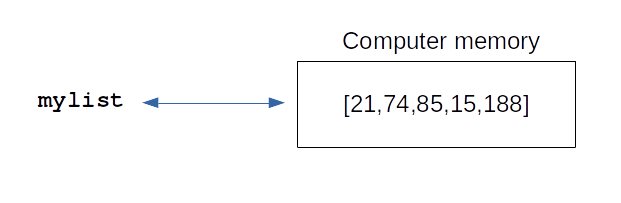
\includegraphics{pic1.png}
\caption{Representation of mylist in the computer memory}
\end{figure}

    \begin{Verbatim}[commandchars=\\\{\}]
{\color{incolor}In [{\color{incolor}60}]:} \PY{k}{for} \PY{n}{item} \PY{o+ow}{in} \PY{n}{mylist}\PY{p}{:} \PY{c+c1}{\PYZsh{} iterate over the list}
             \PY{n+nb}{print} \PY{p}{(}\PY{n}{item}\PY{p}{)}
\end{Verbatim}

    \begin{Verbatim}[commandchars=\\\{\}]
21
74
85
15
188

    \end{Verbatim}

    \begin{Verbatim}[commandchars=\\\{\}]
{\color{incolor}In [{\color{incolor}61}]:} \PY{k}{for} \PY{n}{i}\PY{p}{,} \PY{n}{item} \PY{o+ow}{in} \PY{n+nb}{enumerate}\PY{p}{(}\PY{n}{mylist}\PY{p}{)}\PY{p}{:} \PY{c+c1}{\PYZsh{} enumerate keyword iterates}
                                           \PY{c+c1}{\PYZsh{} returning the item and its index}
             \PY{n+nb}{print} \PY{p}{(}\PY{n}{i}\PY{p}{,} \PY{n}{item}\PY{p}{)}
\end{Verbatim}

    \begin{Verbatim}[commandchars=\\\{\}]
0 21
1 74
2 85
3 15
4 188

    \end{Verbatim}

    \begin{Verbatim}[commandchars=\\\{\}]
{\color{incolor}In [{\color{incolor}62}]:} \PY{n}{secondlist} \PY{o}{=} \PY{p}{[}\PY{p}{]}
         \PY{k}{for} \PY{n}{item} \PY{o+ow}{in} \PY{n}{mylist}\PY{p}{:} \PY{c+c1}{\PYZsh{} create second list using mylist as input}
             \PY{n}{secondlist}\PY{o}{.}\PY{n}{append}\PY{p}{(}\PY{n}{item} \PY{o}{*}\PY{o}{*} \PY{l+m+mi}{2}\PY{p}{)}
         \PY{n}{secondlist}
\end{Verbatim}

\begin{Verbatim}[commandchars=\\\{\}]
{\color{outcolor}Out[{\color{outcolor}62}]:} [441, 5476, 7225, 225, 35344]
\end{Verbatim}
            
    \begin{Verbatim}[commandchars=\\\{\}]
{\color{incolor}In [{\color{incolor}63}]:} \PY{c+c1}{\PYZsh{} for a more compact code the previous lines can be shrinked to}
         \PY{n}{secondlist} \PY{o}{=} \PY{p}{[} \PY{n}{item}\PY{o}{*}\PY{o}{*}\PY{l+m+mi}{2} \PY{k}{for} \PY{n}{item} \PY{o+ow}{in} \PY{n}{mylist}\PY{p}{]}
         \PY{n}{secondlist}
\end{Verbatim}

\begin{Verbatim}[commandchars=\\\{\}]
{\color{outcolor}Out[{\color{outcolor}63}]:} [441, 5476, 7225, 225, 35344]
\end{Verbatim}
            
    \hypertarget{tricky-point-here}{%
\paragraph{Tricky point here !!!}\label{tricky-point-here}}

    \begin{Verbatim}[commandchars=\\\{\}]
{\color{incolor}In [{\color{incolor}64}]:} \PY{n+nb}{print}\PY{p}{(}\PY{n+nb}{sorted}\PY{p}{(}\PY{n}{secondlist}\PY{p}{)}\PY{p}{)} \PY{c+c1}{\PYZsh{} sort returns a new list doesn\PYZsq{}t }
                                   \PY{c+c1}{\PYZsh{} change secondlist itself}
         \PY{n+nb}{print}\PY{p}{(}\PY{n}{secondlist}\PY{p}{)}
\end{Verbatim}

    \begin{Verbatim}[commandchars=\\\{\}]
[225, 441, 5476, 7225, 35344]
[441, 5476, 7225, 225, 35344]

    \end{Verbatim}

    \begin{figure}
\centering
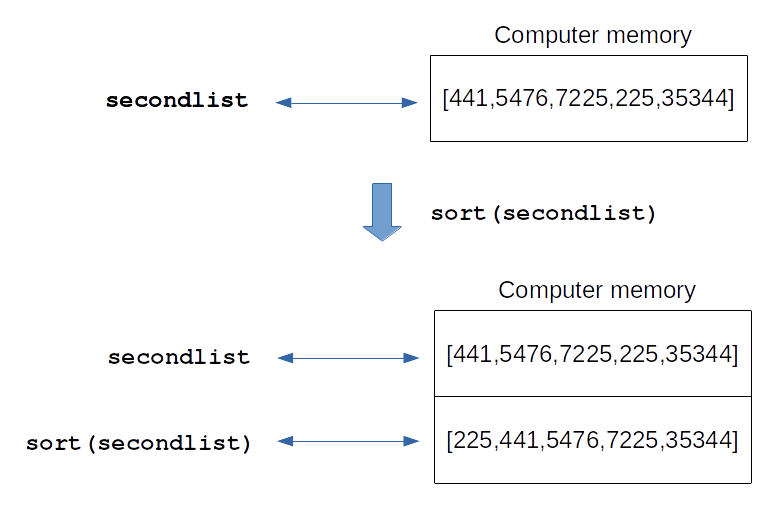
\includegraphics{pic2.png}
\caption{Sorted function returns a new list}
\end{figure}

    \begin{Verbatim}[commandchars=\\\{\}]
{\color{incolor}In [{\color{incolor}65}]:} \PY{n}{secondlist}\PY{o}{.}\PY{n}{sort}\PY{p}{(}\PY{p}{)} \PY{c+c1}{\PYZsh{} instead change secondlist}
         \PY{n}{secondlist}
\end{Verbatim}

\begin{Verbatim}[commandchars=\\\{\}]
{\color{outcolor}Out[{\color{outcolor}65}]:} [225, 441, 5476, 7225, 35344]
\end{Verbatim}
            
    \begin{figure}
\centering
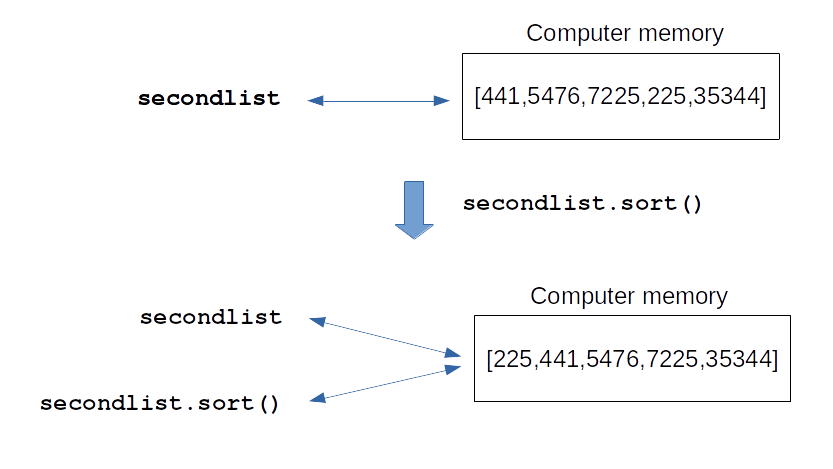
\includegraphics{pic3.png}
\caption{Sort method instead directly changes the current list}
\end{figure}

    \begin{Verbatim}[commandchars=\\\{\}]
{\color{incolor}In [{\color{incolor}66}]:} \PY{n}{thirdlist} \PY{o}{=} \PY{n}{mylist} \PY{c+c1}{\PYZsh{} this is tricky, since variables *point* to objects}
         \PY{n+nb}{print} \PY{p}{(}\PY{n}{mylist}\PY{p}{)}
         \PY{n+nb}{print} \PY{p}{(}\PY{n}{thirdlist}\PY{p}{)}
         \PY{n}{thirdlist}\PY{p}{[}\PY{l+m+mi}{0}\PY{p}{]} \PY{o}{=} \PY{l+m+mi}{0}
         \PY{n+nb}{print} \PY{p}{(}\PY{n}{mylist}\PY{p}{)}
         \PY{n+nb}{print} \PY{p}{(}\PY{n}{thirdlist}\PY{p}{)}
\end{Verbatim}

    \begin{Verbatim}[commandchars=\\\{\}]
[21, 74, 85, 15, 188]
[21, 74, 85, 15, 188]
[0, 74, 85, 15, 188]
[0, 74, 85, 15, 188]

    \end{Verbatim}

    \begin{figure}
\centering
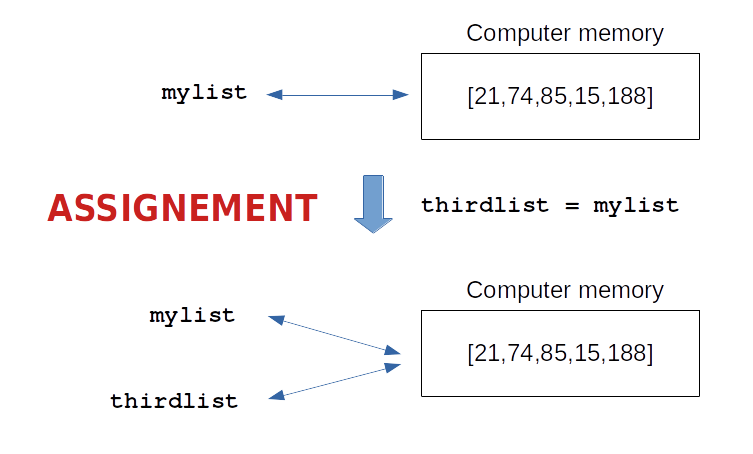
\includegraphics{pic4.png}
\caption{In thist case mylist is assigned to a new variable thirdlist}
\end{figure}

    \begin{Verbatim}[commandchars=\\\{\}]
{\color{incolor}In [{\color{incolor}67}]:} \PY{n}{mylist} \PY{o}{==} \PY{n}{thirdlist} \PY{c+c1}{\PYZsh{} comparison by value, }
                             \PY{c+c1}{\PYZsh{} i.e. they contains the same items}
\end{Verbatim}

\begin{Verbatim}[commandchars=\\\{\}]
{\color{outcolor}Out[{\color{outcolor}67}]:} True
\end{Verbatim}
            
    \begin{Verbatim}[commandchars=\\\{\}]
{\color{incolor}In [{\color{incolor}68}]:} \PY{n}{mylist} \PY{o+ow}{is} \PY{n}{thirdlist} \PY{c+c1}{\PYZsh{} as said before mylist and thirdlist }
                             \PY{c+c1}{\PYZsh{} *point* to the same list}
\end{Verbatim}

\begin{Verbatim}[commandchars=\\\{\}]
{\color{outcolor}Out[{\color{outcolor}68}]:} True
\end{Verbatim}
            
    \begin{Verbatim}[commandchars=\\\{\}]
{\color{incolor}In [{\color{incolor}69}]:} \PY{n}{fourthlist} \PY{o}{=} \PY{n+nb}{list}\PY{p}{(}\PY{n}{mylist}\PY{p}{)} \PY{c+c1}{\PYZsh{} now mylist and fourtfhlist *point* to different list}
         \PY{n}{mylist} \PY{o}{==} \PY{n}{fourthlist}
\end{Verbatim}

\begin{Verbatim}[commandchars=\\\{\}]
{\color{outcolor}Out[{\color{outcolor}69}]:} True
\end{Verbatim}
            
    \begin{Verbatim}[commandchars=\\\{\}]
{\color{incolor}In [{\color{incolor}70}]:} \PY{n}{fourthlist} \PY{o}{=} \PY{n+nb}{list}\PY{p}{(}\PY{n}{mylist}\PY{p}{)} \PY{c+c1}{\PYZsh{} now mylist and fourtfhlist *point* to different list}
         \PY{n}{fourthlist} \PY{o+ow}{is} \PY{n}{mylist}
\end{Verbatim}

\begin{Verbatim}[commandchars=\\\{\}]
{\color{outcolor}Out[{\color{outcolor}70}]:} False
\end{Verbatim}
            
    \begin{figure}
\centering
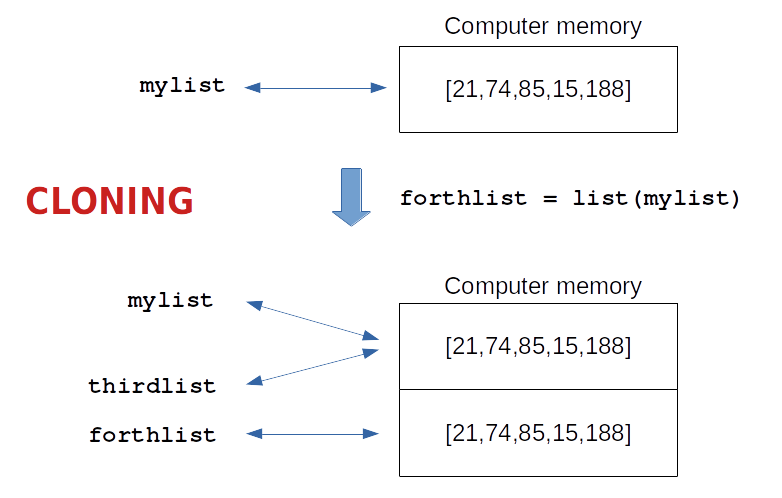
\includegraphics{pic5.png}
\caption{In this case mylist has been cloned into fourthlist}
\end{figure}

List can contain objects of different kind but indices has to be integer

    \begin{Verbatim}[commandchars=\\\{\}]
{\color{incolor}In [{\color{incolor}71}]:} \PY{n}{mixedlist} \PY{o}{=} \PY{p}{[}\PY{l+m+mi}{1}\PY{p}{,} \PY{l+m+mi}{2}\PY{p}{,} \PY{l+s+s2}{\PYZdq{}}\PY{l+s+s2}{b}\PY{l+s+s2}{\PYZdq{}}\PY{p}{,} \PY{n}{math}\PY{o}{.}\PY{n}{sqrt}\PY{p}{]}
         \PY{n+nb}{print} \PY{p}{(}\PY{n}{mixedlist}\PY{p}{)}
\end{Verbatim}

    \begin{Verbatim}[commandchars=\\\{\}]
[1, 2, 'b', <built-in function sqrt>]

    \end{Verbatim}

    \begin{Verbatim}[commandchars=\\\{\}]
{\color{incolor}In [{\color{incolor}72}]:} \PY{n+nb}{print} \PY{p}{(}\PY{n}{mixedlist}\PY{p}{[}\PY{l+m+mi}{0}\PY{p}{]}\PY{p}{)}
         \PY{n+nb}{print} \PY{p}{(}\PY{n}{mixedlist}\PY{p}{[}\PY{l+s+s1}{\PYZsq{}}\PY{l+s+s1}{k}\PY{l+s+s1}{\PYZsq{}}\PY{p}{]}\PY{p}{)}
\end{Verbatim}

    \begin{Verbatim}[commandchars=\\\{\}]
1

    \end{Verbatim}

    \begin{Verbatim}[commandchars=\\\{\}]

        ---------------------------------------------------------------------------

        TypeError                                 Traceback (most recent call last)

        <ipython-input-72-aea4c7f9789e> in <module>()
          1 print (mixedlist[0])
    ----> 2 print (mixedlist['k'])
    

        TypeError: list indices must be integers or slices, not str

    \end{Verbatim}

    \hypertarget{dictionaries}{%
\subsection{Dictionaries}\label{dictionaries}}

Dictionaries are objects which map keys to values. Keys can be (almost)
any kind of object (strings, numbers\ldots{}) and they do not have to be
sequential.

\["apple" \rightarrow 4 \] \["banana" \rightarrow 5 \]

Dictionaries are very flexible so that different keys can be different
type of objects.

    \begin{Verbatim}[commandchars=\\\{\}]
{\color{incolor}In [{\color{incolor}73}]:} \PY{n}{adict} \PY{o}{=} \PY{p}{\PYZob{}}\PY{l+s+s2}{\PYZdq{}}\PY{l+s+s2}{apple}\PY{l+s+s2}{\PYZdq{}}\PY{p}{:} \PY{l+m+mi}{4}\PY{p}{,} \PY{l+s+s2}{\PYZdq{}}\PY{l+s+s2}{banana}\PY{l+s+s2}{\PYZdq{}}\PY{p}{:} \PY{l+m+mi}{5}\PY{p}{\PYZcb{}}
         \PY{n}{adict}\PY{p}{[}\PY{l+s+s2}{\PYZdq{}}\PY{l+s+s2}{apple}\PY{l+s+s2}{\PYZdq{}}\PY{p}{]} \PY{c+c1}{\PYZsh{} values are accessed through their key}
\end{Verbatim}

\begin{Verbatim}[commandchars=\\\{\}]
{\color{outcolor}Out[{\color{outcolor}73}]:} 4
\end{Verbatim}
            
    \begin{Verbatim}[commandchars=\\\{\}]
{\color{incolor}In [{\color{incolor}74}]:} \PY{n}{adict}\PY{p}{[}\PY{l+s+s2}{\PYZdq{}}\PY{l+s+s2}{pear}\PY{l+s+s2}{\PYZdq{}}\PY{p}{]} \PY{c+c1}{\PYZsh{} error ! this key doesn\PYZsq{}t exists}
\end{Verbatim}

    \begin{Verbatim}[commandchars=\\\{\}]

        ---------------------------------------------------------------------------

        KeyError                                  Traceback (most recent call last)

        <ipython-input-74-9d051ebd10de> in <module>()
    ----> 1 adict["pear"] \# error ! this key doesn't exists
    

        KeyError: 'pear'

    \end{Verbatim}

    \begin{Verbatim}[commandchars=\\\{\}]
{\color{incolor}In [{\color{incolor}75}]:} \PY{l+s+s2}{\PYZdq{}}\PY{l+s+s2}{pear}\PY{l+s+s2}{\PYZdq{}} \PY{o+ow}{in} \PY{n}{adict} \PY{c+c1}{\PYZsh{} indeed}
\end{Verbatim}

\begin{Verbatim}[commandchars=\\\{\}]
{\color{outcolor}Out[{\color{outcolor}75}]:} False
\end{Verbatim}
            
    \begin{Verbatim}[commandchars=\\\{\}]
{\color{incolor}In [{\color{incolor}76}]:} \PY{n+nb}{len}\PY{p}{(}\PY{n}{adict}\PY{p}{)}
\end{Verbatim}

\begin{Verbatim}[commandchars=\\\{\}]
{\color{outcolor}Out[{\color{outcolor}76}]:} 2
\end{Verbatim}
            
    \begin{Verbatim}[commandchars=\\\{\}]
{\color{incolor}In [{\color{incolor}77}]:} \PY{n}{adict}\PY{p}{[}\PY{l+s+s2}{\PYZdq{}}\PY{l+s+s2}{banana}\PY{l+s+s2}{\PYZdq{}}\PY{p}{]} \PY{o}{=} \PY{l+m+mi}{2}
         \PY{n+nb}{print} \PY{p}{(}\PY{n+nb}{len}\PY{p}{(}\PY{n}{adict}\PY{p}{)}\PY{p}{)}
         \PY{n+nb}{print} \PY{p}{(}\PY{n}{adict}\PY{p}{)}
\end{Verbatim}

    \begin{Verbatim}[commandchars=\\\{\}]
2
\{'apple': 4, 'banana': 2\}

    \end{Verbatim}

    \begin{Verbatim}[commandchars=\\\{\}]
{\color{incolor}In [{\color{incolor}78}]:} \PY{n}{adict}\PY{p}{[}\PY{n}{math}\PY{o}{.}\PY{n}{log}\PY{p}{]} \PY{o}{=} \PY{n}{math}\PY{o}{.}\PY{n}{exp}
\end{Verbatim}

    \begin{Verbatim}[commandchars=\\\{\}]
{\color{incolor}In [{\color{incolor}79}]:} \PY{n}{adict}\PY{o}{.}\PY{n}{keys}\PY{p}{(}\PY{p}{)} \PY{c+c1}{\PYZsh{} returns all the keys (they are not ordered in any way)}
\end{Verbatim}

\begin{Verbatim}[commandchars=\\\{\}]
{\color{outcolor}Out[{\color{outcolor}79}]:} dict\_keys(['apple', 'banana', <built-in function log>])
\end{Verbatim}
            
    \begin{Verbatim}[commandchars=\\\{\}]
{\color{incolor}In [{\color{incolor}80}]:} \PY{k}{for} \PY{n}{key} \PY{o+ow}{in} \PY{n}{adict}\PY{o}{.}\PY{n}{keys}\PY{p}{(}\PY{p}{)}\PY{p}{:}
             \PY{n+nb}{print} \PY{p}{(}\PY{n}{key}\PY{p}{)}
\end{Verbatim}

    \begin{Verbatim}[commandchars=\\\{\}]
apple
banana
<built-in function log>

    \end{Verbatim}

    \begin{Verbatim}[commandchars=\\\{\}]
{\color{incolor}In [{\color{incolor}81}]:} \PY{k}{for} \PY{n}{value} \PY{o+ow}{in} \PY{n}{adict}\PY{o}{.}\PY{n}{values}\PY{p}{(}\PY{p}{)}\PY{p}{:}
             \PY{n+nb}{print} \PY{p}{(}\PY{n}{value}\PY{p}{)}
\end{Verbatim}

    \begin{Verbatim}[commandchars=\\\{\}]
4
2
<built-in function exp>

    \end{Verbatim}

    \begin{Verbatim}[commandchars=\\\{\}]
{\color{incolor}In [{\color{incolor}82}]:} \PY{k}{for} \PY{n}{item} \PY{o+ow}{in} \PY{n}{adict}\PY{o}{.}\PY{n}{items}\PY{p}{(}\PY{p}{)}\PY{p}{:} \PY{c+c1}{\PYZsh{} items() returns a pair of key, value}
             \PY{n+nb}{print} \PY{p}{(}\PY{n}{item}\PY{p}{)}
\end{Verbatim}

    \begin{Verbatim}[commandchars=\\\{\}]
('apple', 4)
('banana', 2)
(<built-in function log>, <built-in function exp>)

    \end{Verbatim}

    \begin{Verbatim}[commandchars=\\\{\}]
{\color{incolor}In [{\color{incolor}83}]:} \PY{n}{seconddict} \PY{o}{=} \PY{p}{\PYZob{}}\PY{l+s+s2}{\PYZdq{}}\PY{l+s+s2}{watermelon}\PY{l+s+s2}{\PYZdq{}}\PY{p}{:} \PY{l+m+mi}{0}\PY{p}{,} \PY{l+s+s2}{\PYZdq{}}\PY{l+s+s2}{strawberry}\PY{l+s+s2}{\PYZdq{}}\PY{p}{:} \PY{l+m+mi}{1}\PY{p}{\PYZcb{}}
         \PY{n}{adict}\PY{o}{.}\PY{n}{update}\PY{p}{(}\PY{n}{seconddict}\PY{p}{)} \PY{c+c1}{\PYZsh{} update adict with the items in seconddict}
         \PY{n}{adict}
\end{Verbatim}

\begin{Verbatim}[commandchars=\\\{\}]
{\color{outcolor}Out[{\color{outcolor}83}]:} \{'apple': 4,
          'banana': 2,
          <function math.log>: <function math.exp>,
          'watermelon': 0,
          'strawberry': 1\}
\end{Verbatim}
            

    \subsection{Exercises}\label{exercises}

\subsubsection{Exercise 1.1}\label{exercise-1.1}

\begin{itemize}
\tightlist
\item
  What is a built-in function that Python uses to iterate over a number
  sequence?
\item
  What is a string in Python?
\item
  What does the continue do in Python?
\item
  What is the purpose of end in Python?
\item
  When should you use the break in Python?
\item
  What is a dictionary in Python programming?
\item
  What is the use of the dictionary in Python?
\item
  How do you create a dictionary in Python?
\item
  How do you read from a dictionary in Python?
\item
  How do you traverse through a dictionary object in Python?
\item
  How do you add elements To a dictionary in Python?
\item
  How do you delete elements Of a dictionary in Python?
\item
  How do you check the presence of a key in a dictionary?
\item
  What is the syntax for list comprehension in Python?
\item
  What is the syntax for dictionary comprehension in Python?
\item
  How do you write a conditional expression in Python?
\item
  Which Python function will you use to convert a number to a string?
\end{itemize}
    

\section{Advanced hints}\label{advanced-hints}

If you would like to know much \textbf{more} about python during the
course without the EDX site you can look these videos during the course
in your spare time:

Some more information about different kind of languages:
https://www.youtube.com/watch?v=9oYFH4OmYDY

Basic data types: https://www.youtube.com/watch?v=XIjrEt2lz1U

Variables: https://www.youtube.com/watch?v=z2NLjdfxEyQ

Branching: https://www.youtube.com/watch?v=8vr3nyg5QcM

Tuples: https://www.youtube.com/watch?v=CwZyWaap5Z8

Lists: https://www.youtube.com/watch?v=eMyWO0tcxKg

List Operations: https://www.youtube.com/watch?v=rQBho4-bI3o

Mutation, Aliasing, Cloning: https://www.youtube.com/watch?v=2SRXg8Or-Pc

Functions as Objects: https://www.youtube.com/watch?v=pheM3rVmGMU

Dictionaries: https://www.youtube.com/watch?v=elSt5hke-Rs


    % Add a bibliography block to the postdoc
    

    \end{document}
